\section{Indledning}

I projektforløbet er der løbende blevet udført test. Indledningsvis udføres enhedstest i takt med nye enheder udvikles, senere laves integrationstest der tester kommunikation og samarbejde mellem flere enheder og til sidst udføres accepttest, der bruges til at teste det samlede system. Nedenfor beskrivelses de forskellige tests:


\subsection{Enhedstest} 
\vspace{-0.5cm}
Enhedstest er en testmetode der benyttes til at isolere og teste systemets enkelte enheder. Enhedstest udføres løbende i takt med nye enheder udvikles. Testene udarbejdes for at sikre kvalitet, funktionalitet og grænseflader af de nyudviklede enheder. 

Hovedformålet med enhedstest er at teste tidligt i projektforløbet for at opdage eventuelle fejl og mangler. Hvilket i sidste ende sparer gruppen for meget tid og besvær, da fejl og mangler er svære og mere tidskrævende at rette sent i et projektforløb.

Figur \ref{fig:test_forlob} illustrerer hvordan mange fejl kan findes ved brug af enhedstest. Fejl der ellers "først" var blevet fundet når systemets enheder blev koblet sammen.
\vspace{-0.4cm}
\begin{figure}[H]
	\centering
	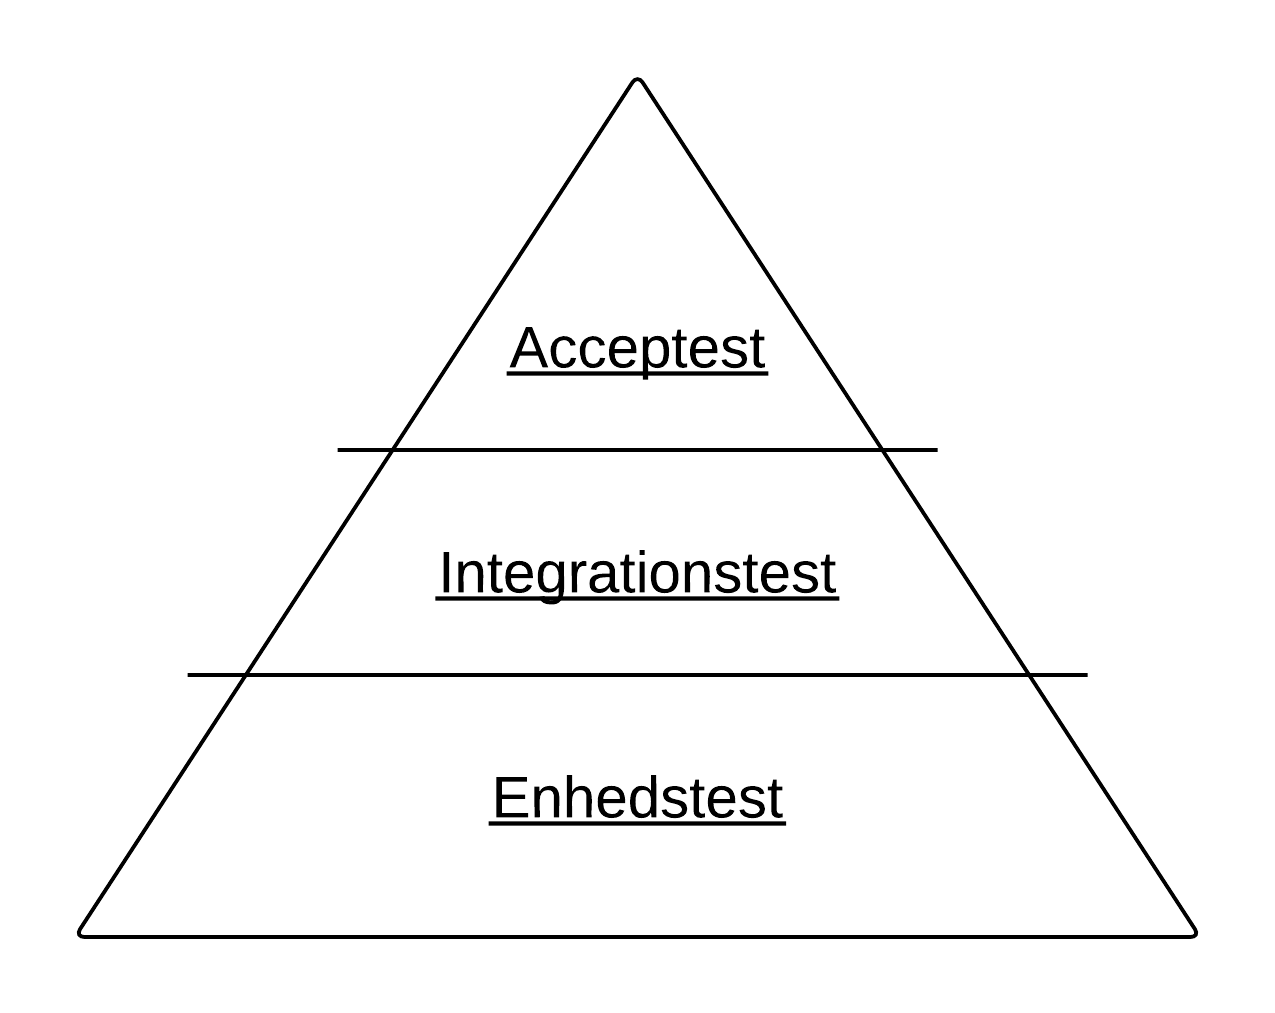
\includegraphics[width=0.5\textwidth]{Billeder/Test/forlob.png}
	\vspace{-0.4cm}
	\caption{Mængde af fejl fundet ved test}
	\label{fig:test_forlob}
\end{figure}

\vspace{0.5cm}

Enhedstest bygges som regel op efter AAA-modellen\footnote{http://c2.com/cgi/wiki?ArrangeActAssert}.\\ 
\textbf{A}rrange: Opsætning af input til test og håndtering af afhængigheder. \\
\textbf{A}ct: Hardware/software enhed under test stimuleres. \\
\textbf{A}ssert: Der kigges på output og det afgøres om testen er succesfuld eller ej.

På  figur \ref{fig:aaa} ses et eksempel på software test efter AAA modellen. I testen bliver der testet om den korrekte metode bliver kaldt når bruger prøver at logge in på webapplikationen. 

\begin{figure}[H]
	\centering
	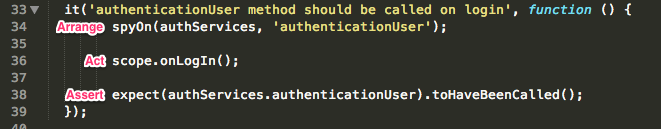
\includegraphics[width=0.75\textwidth]{Billeder/Test/aaa.png}
	\caption{AAA eksempel}
	\label{fig:aaa}
\end{figure}

\newpage

\subsection{Integrationstest} 
Integrationstest bruges til at teste kobling mellem to eller flere enheder. Integrationstest bruges til at kontrollere om enhederne under test kan kommunikere og arbejde sammen. 

Integrationstest af hardware og tilhørende software klasser er udført efter Collaboration modellen, mens software til server og webapplikation er integrationstestet efter metoderne buttom-up, top-down og collaboration. \\

\vspace{-0.4cm}

\textbf{Collaboration}\\
Når der testes efter collaboration samles en række enheder. Inden sammenkobling udgør hver enhed en lille klump funktionalitet, men tilsammen udgør enhederne en væsentlig del af systemts samlede funktionalitet.
På figur \ref{fig:Collaboration} illustreres et eksempel på collaboration.

\vspace{-5pt}
%kommentar
\begin{figure}[H]
	\centering
	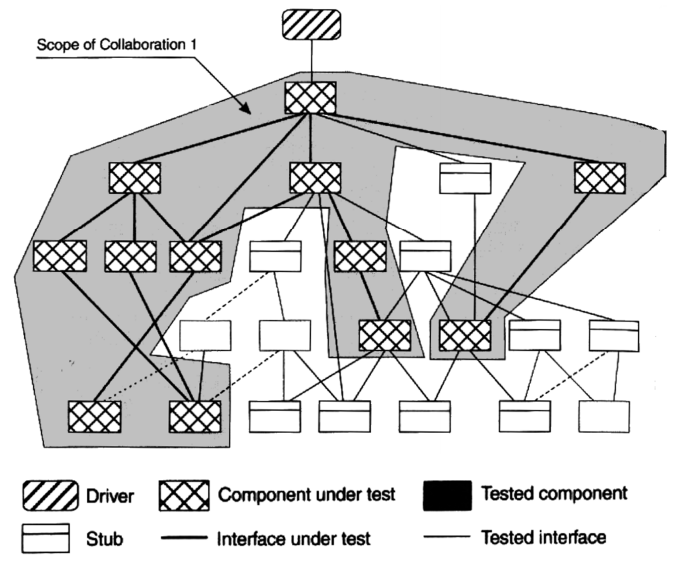
\includegraphics[width=0.6\textwidth]{Billeder/Test/collaboration.png}
	\vspace{-5pt}
	\caption{Collaboration}
	\label{fig:Collaboration}
\end{figure}


\textbf{Button-Up}\\
På figur \ref{fig:Buttom_up} ses et eksempel på buttom up testing. Figuren viser hvordan systemets mest grundlæggende klasser er først testet og derefter bliver der testet op igennem systemet. 

%kommentar
\begin{figure}[H]
	\centering
	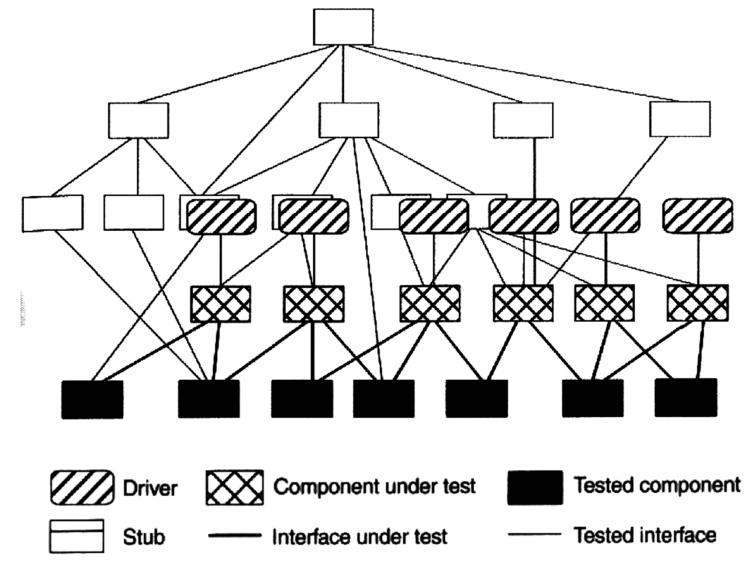
\includegraphics[width=0.6\textwidth]{Billeder/Test/buttom-up.png}
	\vspace{-5pt}
	\caption{Buttom up}
	\label{fig:Buttom_up}
\end{figure}

\newpage

\textbf{Top-Down}\\
På figur \ref{fig:Top_down} ses et eksempel på top down testing. Figuren vises hvordan systemets top klasser er testet først og derefter testet ned igennem klasserne.

%kommentar
\begin{figure}[H]
	\centering
	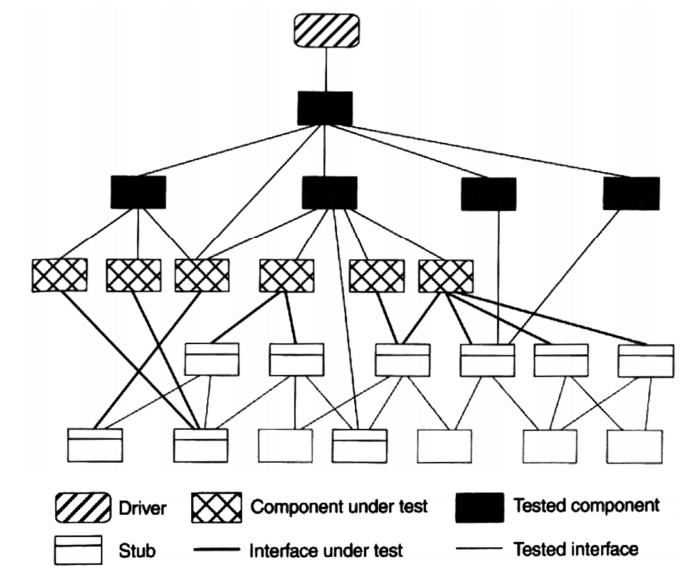
\includegraphics[width=0.65\textwidth]{Billeder/Test/top-down.png}
	\vspace{-5pt}
	\caption{Top down}
	\label{fig:Top_down}
\end{figure}

\vspace{1.5cm}

\subsection{Accepttest} 
Accepttesten er en todelt test der tester systemet som helhed. 
Først udføres accepttest af funktionelle krav og dernæst testes ikke-funktionelle krav.
Accepttest af funktionelle krav foregår via en gennemgang af use cases, som bruges til at kontrollere systemets funktionalitet. Ikke-funktionelle krav bruges til at teste systemspecifikationer.  
